% ---
% Capitulo de revisão de literatura
% ---

\chapter{Revisão de Literatura}
\label{cap:revisaoliteratura}

% Para o bom entendimento do trabalho, é necessário que se explique os nomes, conceitos, e ferramentas utilizadas para o desenvolvimento deste trabalho.

Primeiramente, apresentamos conceitos linguísticos na sessão \ref{sec:parsing}. Em seguida, na sessão \ref{sec:treebank}, estudamos os \textit{treebanks}: o que são, suas estruturas, e os \textit{treebanks} utilizados neste trabalho, tanto os que serão transduzidos, como o \textit{treebank} de referência. Por fim, em \ref{sec:parser}, explicamos os  \textit{parsers}: seu funcionamento, o \textit{parser} que utilizaremos para o estudo, alguns \textit{parsers} da língua portuguesa, e mostramos algumas formas de avaliação.

\section{Análise Sintática (\textit{Parsing})}
\label{sec:parsing}

Análise sintática, ou \textit{parsing}, é uma técnica que possui importância principalmente em duas áreas de conhecimento. A primeira, no campo do processamento de Linguagens de Computação. Na segunda, no campo do Processamento de Linguagens Naturais.

Sobre linguagens de computação, \citeonline[p~39]{aho2008compiladores} definem a análise sintática como \textquote{O processo para determinar como uma cadeia de terminais pode ser gerada por uma gramática}. Terminais são, na sua definição, (\textit{\Ibidem[p~27]{aho2008compiladores}}) \textquote{os símbolos elementares da linguagem, definidos pela gramática}. Sobre gramática, (\textit{\Ibidem[p~39]{aho2008compiladores}}) \textquote{descreve [\ldots] a estrutura hierárquica da maioria das construções de linguagens [\ldots]}. 

Já sobre Processamento de Linguagem Natural (que será dado foco neste trabalho), como descrito por \citeonline[p~33]{charniak97statistical}, \textit{parsing} é \textquote{\textit{the process of assigning a phrase marker to a sentence}} \footnote{\textquote{O processo de atribuir marcadores de frase a uma sentença}. Tradução própria}. Por exemplo, na frase \textquote{\textit{o cachorro late}}, \textit{o} pode ser marcado como artigo, \textit{cachorro} como substantivo, \textit{late} como verbo. \textit{O cachorro}, juntos, formam um sintagma nominal. O verbo, sozinho, faz parte de um sintagma verbal. E ambos formam a sentença. Como fica mais claro na Figura \ref{fig:parse-simple}.

\begin{center}
    \begin{figure}[h!]
    \centering
    % \includegraphics{}
    \begin{forest}
        [S
            [NP
                [artigo
                    [\textit{o}]
                ]
                [substantivo
                    [\textit{cachorro}]
                ]
            ]
            [VP
                [verbo
                    [\textit{late}]
                ]
            ]
        ]
    \end{forest}
    \caption[Exemplo de árvore simples]{Exemplo de árvore simples (Adaptado de \citeonline[p~34]{charniak97statistical})}
    \label{fig:parse-simple}
\end{figure}
\end{center}

A esta estrutura damos o nome de \textit{árvore de derivação}, \textit{árvore}, ou \textit{parse}.

Para sentenças simples, este é um trabalho simples. Porém, muito facilmente uma frase pode gerar mais de uma árvore, ou seja, gerar uma ambiguidade sintática\footnote{Nota: Não haverá foco na ambiguidade lexical neste trabalho.}, como no exemplo usado por \citeonline[p~10]{paganiavaliaccao}, na Figura \ref{fig:parse-ambiguity}

\begin{center}
    \begin{figure}[h!]
    \centering
    % \includegraphics{}
    Para a sentença \textquote{\textit{Arlindo tirou os pés da mesa}}:
    
    \textbf{a)}
    \begin{forest}
        [S
            [SN
                [\textit{Arlindo}]
            ]
            [SV
                [V
                    [\textit{tirou}]
                ]
                [SN
                    [SN
                        [\textit{os pés}]
                    ]
                    [SP
                        [\textit{da mesa}]
                    ]
                ]
            ]
        ]
    \end{forest}
    
    \textbf{b)}
    \begin{forest}
        [S
            [SN
                [\textit{Arlindo}]
            ]
            [SV
                [V
                    [\textit{tirou}]
                ]
                [SN
                    [\textit{os pés}]
                ]
                [SP
                    [\textit{da mesa}]
                ]
            ]
        ]
    \end{forest}
    \textbf{c)}
    \begin{forest}
        [S
            [SN
                [\textit{Arlindo}]
            ]
            [SV
                [SV
                    [V
                        [\textit{tirou}]
                    ]
                    [SN
                        [\textit{os pés}]
                    ]
                ]
                [SP
                    [\textit{da mesa}]
                ]
            ]
        ]
    \end{forest}
    
    \caption[Exemplo de ambiguidade entre árvores]{Exemplo de ambiguidade entre árvores (Adaptado de \citeonline[p~10]{paganiavaliaccao})}
    \label{fig:parse-ambiguity}
\end{figure}
\end{center}

Além da ambiguidade, existe outro problema: a quantidade de árvores incoerentes. Como destaca \citeonline[p~33]{charniak97statistical}, o exemplo 
\textquote{\textit{[\ldots] Implica que podemos atribuir pelo menos um significado semi-plausível para toda árvore possível. Para a maioria das gramáticas [\ldots], este não é o caso}
\footnote{No original: \textquote{[\ldots] implies that we can assign at least a semiplausible meaning to all the possible parses. For most grammars [\ldots], this is not the case.} Tradução própria.}}.
Ou seja, é necessário filtrar as árvores com real relevância e que mais se aproximem de uma estrutura correta.

Nesse ponto, existem métodos que resolvam essa ambiguidade, como as Gramáticas Lives de Contexto Probabilísticas e a classificação lexicalizada. Ambos serão abordados, respctivamente, nas sessões \ref{subsec:statisticalparsing} e \ref{subsec:lexParsing}.

O leitor pode se questionar qual a utilidade de \textit{parsing}, e do seu estudo. \citeonline{Manning1999FoundationsNLP} dedicam alguns capítulos para demonstrar seu uso e técnicas\ como Tradução de Máquina, Agrupamento (\textit{clustering}), Recuperação de Informação e Categorização de Textos. Entrar nestes assuntos escaparia ao escopo deste trabalho, mas recomendamos a leitura\footnote{\cite[capítulos~13,14,15,16]{Manning1999FoundationsNLP}}.

% Apesar de uma ferramenta muito útil e desafiadora, \citeonline[p~457]{Manning1999FoundationsNLP} destacam:
% \textquote{\textit{Partly because parsers do not perform well enough yet, parsing has rarely been applied to higher-level tasks like speech recognition and language understanding}}
% \footnote{\textquote{Em partes por ainda não performarem bem o bastante ainda, \textit{parsing} raramente vem sendo aplicado para tarefas de alto nível como reconhecimento de fala e compreensão de linguagem}. Tradução própria.}. 

% ---------------------------------------------------------

\subsection{Etiquetas Morfosintáticas - Part of Speech Tags}
\label{subsec:POStags}

Sintaticamente falando, palavras podem ser agrupadas em classes (ou grupos) que demonstrem seu comportamento sintático. Tais classes podem ser chamadas de Categorias Sintáticas, ou Categorias Gramaticais. Mesmo Classes. Exemplos de classes são \textit{verbo}, \textit{substantivo}, \textit{adjetivo}, \textit{artigo} etc. Outra forma de se referir a tais classes, é chamando-as de \textquote{\textit{Part of Speech}}\footnote{Parte do Discurso} (POS).

% Como saber se palavras diferentes pertencem ao mesmo grupo? 
\cite[p~81]{Manning1999FoundationsNLP} \textquote{O teste mais básico para palavras pertencentes à mesma classe é o teste de substituição}
\footnote{No original: \textquote{\textit{The most basic test for words belonging to the same class is the substitution test.}} Tradução própria.}.
Podemos ver um exemplo na Figura \ref{fig:substTest}.

\begin{center}
\begin{figure}[h!]
    \centering
    % \includegraphics{}
    \begin{tabular}{c c c}
        A &
        %  \[ 
        \begin{math}
            \left \{
                \begin{tabular}{c}
                    casa\\
                    pessoa\\
                    mulher\\
                    criança\\
                    Bolsa de Valores\\
                    pena\\
                \end{tabular}
            \right \}
            % \] 
        \end{math}
            & caiu.\\
    \end{tabular}
    
    \caption[Teste de Substituição]{Teste de Substituição}
    \label{fig:substTest}
\end{figure}
\end{center}

Na Figura \ref{fig:substTest}, demonstramos o teste da substituição para substantivos. Note que palavras podem ter mais de uma POS. Por exemplo, \textit{casa} pode ser um substantivo (NN), ou a terceira pessoa do singular do verbo \textquote{casar} (VBZ
\footnote{Essa é uma tag do Penn Treebank, usada de maneira direta. Em \ref{subsec:PennTB} explicamos melhor este \textit{treebank}, e suas possíveis traduções no capítulo \ref{cap:desenv}.}
). Sistemas que fazem análise sintática de sentenças atribuem um rótulo a cada palavra que represente a sua classe gramatical. Esta marca é chamada de Etiqueta Morfossintática (ou \textit{POS tag}, no inglês).

Palavras podem ser de duas categorias principais, citadas por \citeonline[p~82]{Manning1999FoundationsNLP}:
\begin{quote}
    \textquote{As categorias abertas, ou lexicais, são aquelas como substantivos, verbos e adjetivos, que tem um grande número de membros, e nos quais novas palavras são comumente adicionadas. As fechadas, ou funcionais, são categorias como preposições e artigos (contendo palavras como \textit{de, em, o, um}) que tem apenas poucos membros, e cujos membros normalmente tem um claro uso gramatical}
    \footnote{No original: \textquote{\textit{The open or lexical categories are ones like nouns, verbs and adjectives which have a large number of members, and to which new words are commonly added. The closed or functional categories are categories such as prepositions and determiners (containing words like of, on, the, a) which have only a few members, and the members of which normally have a clear grammatical use.}}. Tradução própria.}
\end{quote}
Podemos complementar essa ideia com a Tabela \ref{tab:classesPalavras}, apresentada por \citeonline[p~55]{Castilho2010gramatica}:

\begin{center}
\begin{table}[h!]
    \centering
    \begin{tabular}{|c|c|}
        \hline
        Palavras Variáveis & Palavas Invariáveis\\\hline
        Verbo & Advérbio\\\hline
        Substantivo & Preposição\\\hline
        Artigo & Conjunção\\\hline
        Pronome & Adjetivo\\\hline
    \end{tabular}
    \caption[Classes de Palavras no Português]{Classes de Palavras no Português. Adaptada de \citeonline[p~55]{Castilho2010gramatica}}
    \label{tab:classesPalavras}
\end{table}
\end{center}

Algumas POS tags serão descritas com mais detalhes quando forem abordados o Penn Treebank (\ref{subsec:PennTB}), e \textit{treebanks} para o Português (\ref{subsec:tbPortugues}).

% ---------------------------------------------------------

\subsection{Análise de Constituinte e Sintagma}
\label{subsec:analiseConstSintagma}

% Análise de constituinte (\textit{Constituency Parsing}) desempenha papel importante em muitas aplicações de linguagem natural. 
% % \citeonline{zhang2017headSelection} relembram que parsers são usados em
% \textit{Parsers} podem ser usados em \citeonline[p~625]{zhang2017headSelection} \textquote{\textit{relation extraction, machine translation, language modeling and ontology construction}}
% \footnote{Extração de relações, tradução de máquina, modelagem de linguagem, e construção de ontologias. Tradução própria.}, para citar exemplos. 
% Eles também destacam que esta forma de \textit{parsing} \textquote{\textit{represent syntactic information as a set of head-dependent relational arcs, typically constrained to form a tree}}
% \footnote{\textquote{Representa informação sintática como um um conjunto de arcos relacionais núcleo-dependente, tipicamente forçado a formar uma árvore}. Tradução própria.}. 
% Em outras palavras, remetendo à imagem \ref{fig:parse-simple} a relação \textit{o} e \textit{cachorro} demonstra o substantivo (cachorro) como núcleo (ou \textit{head}), e o artigo (o) como dependente (\textit{dependent}). 
Em qualquer linguagem, palavras não são ditas ao acaso. Existe uma ordem, e regras, para que elas sejam bem emitidas, e bem recebidas. Um conceito fundamental sobre tal ordenação é a ideia que palavras se agrupam de forma hierárquica. 
Esta estrutura pode ser visualizada na Figura \ref{fig:constituency-tree},
\begin{center}
\begin{figure}[!ht]
    \centering
    \begin{forest}
        [S [NP [PRS Ele]] [VP [V mora] [ADVP [ADV muito] [ADVP [ADV perto] [PP [P de\_] [NP [ART o] [N centro]]]]]]]
    \end{forest}
    \caption[Exemplo de árvore de Constituência]{Exemplo de árvore de Constituência. Adaptado da sentença aTSTS-002/80, do CINTIL}
    \label{fig:constituency-tree}
\end{figure}
\end{center}
Para entender esta hierarquia, é essencial entender o conceito de sintagma. 

O sintagma (ou \textit{phrase}) é, de acordo com \citeonline[p~55]{Castilho2010gramatica},
\begin{quote}
    \textquote{a quarta unidade gramatical na hierarquia descritivista
    \footnote{Os anteriores são: o Fonema, a Sílaba, o Morfema}.
    Trata-se de uma associação de palavras articuladas à volta de cinco dentre elas: o verbo, o substantivo, o adjetivo, o advérbio e a preposição. [\ldots] A classe de palavras que nucleariza o sintagma dá-lhe o nome, e assim teremos o sintagma nominal (SN), o sintagma verbal (SV), o sintagma adjetival (SAdj), o sintagma adverbial (SAdv) e o sintagma preposicionado (SP)}
    \footnote{Este trabalho baseou-se no \textit{tagset} do \textit{Penn Treebank}, que será melhor explicado na sessão \ref{subsec:PennTB}. Salvo exceções, serão utilizados neste trabalho os rótulos para sintagmas (\textit{phrase tag}) equivalentes ao do Penn. Que conste : \textit{noun phrase} (NP), \textit{verbal phrase} (VP), \textit{adjective phrase} (ADJP), \textit{adverb phrase} (ADVP), \textit{prepositional phrase} (PP)}. 
\end{quote}
E, \textquote{Os sintagmas exemplificam a propriedade de \textquote{constituência}, isto é, a capacidade linguística de organizar expressões dotadas de uma margem esquerda, um núcleo e uma margem direita} (\textit{\Ibidem[p~55]{Castilho2010gramatica}}).

\cite{NLPConstParsing} destaca que \textquote{\textit{Constituency parsing aims to extract a constituency-based parse tree from a sentence that represents its syntactic structure according to a phrase structure grammar}}\footnote{\textquote{Análise de Constituência visa extrair uma árvore baseada em constituencia de uma sentença que represente sua estrutura sintática de acordo com uma gramática de estrutura frasal}. Tradução própria.}, ou seja, uma árvore de constituintes (ou árvore de constituência - \textit{constituency parse}). Esta árvore demonstra a relação hierárquica da sentença e dos seus elementos. Como destacam \citeonline[p~93]{Manning1999FoundationsNLP},
\begin{displayquote}
    \textquote{\textit{One fundamental idea is that certain groupings of words behave as constituents. Constituents can be detected by their being able to occur in various positions, and showing uniform syntactic possibilities for expansion.}}
    \footnote{\textquote{Uma ideia fundamental é que certos agrupamentos de palavras se comportam como constituintes. Constituintes podem ser detectados por serem capazes de ocorrer em várias posições, e mostrar possibilidades sintáticas uniformes para expansão}. Tradução própria.}
\end{displayquote}
Sobre a mudança de posição, podemos exemplificar como:
\begin{itemize}
    \item Eu fui no mercado comprar maçãs
    \item Comprar maçãs, no mercado, eu fui
    \item Eu fui comprar maçãs, no mercado
\end{itemize}
Sobre a expansão de um constituinte, seria como na Tabela \ref{tab:rel_sintagma}:

\begin{center}
\begin{table}[!ht]
    \centering
    \begin{tabular}{ c c c }
        Ele & \textbf{COMPROU} & isso \\ 
        Ontem ele & \textbf{COMPROU} & maçã \\  
        Ele foi ontem e & \textbf{COMPROU} & uma maçã \\
        Ele foi na loja e & \textbf{COMPROU} & uma torta de maçã
    \end{tabular}
    \caption{Exemplo de expansão de constituinte}
    \label{tab:rel_sintagma}
\end{table}
\end{center}

Elementos que podem ser substituídos por outro numa posição sintática apresentam um \textit{relacionamento paradigmático}. Duas palavras que podem formar um sintagma possuem \textit{relação sintagmática}.

\subsection{Estrutura Frasal}
\label{subsec:estrFrasal}

\citeonline[p~93]{Manning1999FoundationsNLP} dizem 
\textquote{\textit{Syntax is the study of the regularities and constraints of word order and phrase structure}}
\footnote{\textquote{Sintaxe é o estudo das regularidades e restrições da ordem das palavras e estrutura frasal}. Tradução própria.}.
Isso é importante, pois as palavras não estão simplesmente \textquote{jogadas} numa frase. Sua ordem, sua morfologia, tudo influencia para o significado que ela expressa.

Já abordamos em \ref{subsec:analiseConstSintagma} o conceito de constituintes, que é fundamental para esse estudo. Vamos falar, agora, um pouco mais sobre estruturas.

Gramáticas como a inglesa tem a estrutura mais estática, ou seja, as palavras têm posições bem definidas, que implicam no seu significado. No exemplo citado por \citeonline[p~85]{Manning1999FoundationsNLP},
\begin{itemize}
    \item \textit{Mary gave Peter a book}
    \item \textit{Peter gave Mary a book}
\end{itemize}
Informam exatamente quem deu o livro a quem. A ordem das palavras determina a categoria da frase. No caso:
\begin{itemize}
    \item Forma base: Sujeito - Verbo - Objeto
    \begin{itemize}
        \item \lbrack The children\rbrack \lbrack should\rbrack \lbrack eat spinach\rbrack
    \end{itemize}
    \item Interrogativo: Verbo - Sujeito - Objeto
    \begin{itemize}
        \item \lbrack Should\rbrack \lbrack the children\rbrack \lbrack eat spinach\rbrack?
    \end{itemize}
    \item Imperativo: Verbo - Objeto
    \begin{itemize}
        \item \lbrack Eat\rbrack \lbrack spinach\rbrack!
    \end{itemize}
\end{itemize}
Já línguas como o Latim ou o Russo podem posicionar as palavras em qualquer posição, sem perda de significado. São chamadas \textquote{Free Word Order Language}
\footnote{\textquote{Linguagem de livre ordem das palavras}. Tradução própria}. Tais linguagens utilizam outros marcadores para definir o significado, e utilizam a ordem para indicar estrutura de discurso. Exemplo:
\begin{itemize}
    \item Pedro deu o livro a Maria
    \item Maria deu o livro a Pedro
    \item A Maria, Pedro deu o Livro
\end{itemize}

Para reproduzir o padrão de sentenças, podemos nos valer das regras de reescrita. \cite[p~96]{Manning1999FoundationsNLP}
\textquote{\textit{A rewrite rule has the form \textquote{category $\to$ category*} and states that the symbol on the left side can be rewritten as the sequence of symbols on the right side}}
\footnote{\textquote{Uma regra de reescrita tem a forma \textquote{categoria $\to$ categoria*} e declara que o símbolo do lado esquerdo pode ser reescrito com a sequência de símbolos no lado direito}. Tradução própria.}.
Ou seja, para quem já está familiarizado com o estudo de teoria dos autômatos, seriam as regras de produção ou reescrita. \cite[p~171]{hopcroft2003automataTheory} define uma produção como:
\begin{itemize}
    \item \textquote{Uma variável que está sendo (parcialmente) definida pela produção. Esta variável é geralmente chamada \textquote{núcleo} da produção.}
    \footnote{No original: \textquote{\textit{A variable that is being (partially) defined by the production. This variable is often called the \textit{head} of the production.}} Tradução própria.}
    \item \textquote{O símbolo da produção $\rightarrow$.}
    \footnote{No original: \textquote{\textit{The production symbol $\rightarrow$.}} Tradução própria.}
    \item \textquote{Uma cadeia de caracteres de zero ou mais terminais e variáveis. Essa cadeia, chamada o corpo da produção, representa o modo de formar cadeias na linguagem da variável do núcleo.}
    \footnote{\textquote{\textit{A string of zero or more terminals and variables. This string, called the \textit{body} of the production, represents one way to form strings in the language of the variable of the head.}} Tradução própria.}
\end{itemize}

As  produções dependem apenas da variável a ser reescrita (no nosso caso, a categoria sintática). Portanto, temos uma Gramática Livre de Contexto (GLC, ou CFG em Inglês).

\subsection{Classificação Estatística (\textit{Statistical Parsing})}
\label{subsec:statisticalparsing}

Como dito em \ref{sec:parsing}, uma das dificuldades no processo de \textit{parsing} é a resolução de ambiguidades. \cite[33]{charniak97statistical}
\textquote{maior parte das árvores que gramáticas com ampla cobertura encontram [\ldots] não fazem sentido.}
\footnote{No original: \textquote{\textit{most of the parses that wide-coverage grammars find are [\ldots] pretty senseless.}} Tradução própria.}
Isto exige uma estratégia para, não só identificar a sentença mais provável, como rejeitar classificações de baixa qualidade. 

Uma estratégia possível é o uso da estatística. Como já visto em \ref{sec:parsing} e \ref{subsec:analiseConstSintagma}, a estrutura de um \textit{parse} é uma árvore de derivação, em que os nós terminais (folhas) são as palavras, e os nós não-terminais são referentes aos sintagmas, e compõem a estrutura de derivação e constituência. Pode-se, então, catalogar todas as possíveis derivações de cada sintagma, criando uma \textit{gramática}. Tais derivações são chamadas de regras.

Determinar qual regra utilizar em cada derivação para classificar uma sentença se torna a questão a ser resolvida. Atribuindo-se um valor de probabilidade para cada regra, pode-se, então, selecionar as regras mais prováveis para uma dada sentença. \cite[p~37]{charniak97statistical} 
\textquote{Classificação estatística funciona atribuindo probabilidades à possíveis árvores de uma sentença, localizando a árvore mais provável, e então apresentando tal árvore como resposta.}
\footnote{No original: \textquote{\textit{Statistical parsers work by assigning probabilities to possible parses of a sentence, locating the most probable parse, and then presenting the parse as the answer.}} Tradução própria.}

Com isto, pode-se intuir uma estrutura simples, uma Gramática Livre de Contexto com probabilidades atribuidas às suas regras. \cite[p~382]{Manning1999FoundationsNLP}
\begin{quote}
    \textquote{O modelo probabilístico mais simples para incorporação recursiva é uma PCFG, uma Gramática Livre de Contexto Probabilística (às vezes também chamada Estocástica), que é simplesmente uma GLC com probabilidades adicionadas às regras, indicando o quão prováveis diferentes reescritas são.}
    \footnote{No original: \textquote{\textit{The simplest probabilistic model for recursive embedding is a PCFG, a Probabilistic (sometimes also called Stochastic) Context Free Grammar which is simply a CFG with probabilities added to the rules, indicating how likely different rewritings are.}} Tradução própria.}
\end{quote}
    
Deste modo, dada uma sentença $s$, e uma possível árvore $\pi$, sendo $c$ os constituintes da árvore, e $r(c)$ a regra usada para expandir $c$, temos a equação \ref{eq:pcfg_simples}.
\begin{center}
    \begin{equation}
\label{eq:pcfg_simples}
    p(s,\pi) = \prod_c{p(r(c))}
\end{equation}   
\end{center}
Ou seja, a probabilidade de uma dada árvore, para uma sentença específica, é o produto das probabilidades de todas as regras de expansão desta mesma árvore.

Existem várias vantagens nas PCFGs. A estrutura de gramática livre de contexto é bastante conhecida tanto por cientistas da computação, como por linguistas. Também, como visto em  \cite[p~38]{charniak97statistical}, algoritmos baseados em PCFG são tão eficientes quanto algoritmos não-estatísticos baseados em gramáticas.

Para se criar uma PCFG, o procedimento é como segue: deve-se ler árvores previamente classificadas (e consideradas corretas). Neste processo, deve-se anotar a quantidade de regras utilizadas. No exemplo de (\textit{\Ibidem[p~38]{charniak97statistical}}):
\begin{quote}
    \textquote{É possível ler todas as regras necessárias dessa maneira. Além disso, podemos atribuir as probabilidades às regras contando com que frequência cada regra é usada. Por exemplo, se a regra $np \rightarrow det\, noun$ é usada, digamos, 1000 vezes, e regras gerais de $np$ são usadas 60.000 vezes, então atribuímos à essa regra a probabilidade $1,000/60,000 = .017$}
    \footnote{No original: \textquote{\textit{It is possible to read off all the necessary rules in this fashion. Furthermore, we can assign probabilities to the rules by counting how often each rule is used. For example, if the rule $np \rightarrow det\, noun$ is used, say, 1,000 times, and overall $np$ rules are used 60,000 times, then we assign this rule the probability $1,000/60,000 = .017$.}}. Tradução própria.}
\end{quote}
Para catalogar as regras necessárias para uma gramática, é necessário um conjunto de sentenças / árvores pré-classificadas. São chamados de bancos de árvores, florestas sintáticas, ou \textit{treebanks}, que serão comentados em \ref{sec:treebank}. Um dos mais populares entre eles, o \textit{Penn Treebank} (ou PTB), é abordado em \ref{subsec:PennTB}. Preferencialmente, esses conjuntos tem que ter uma quantidade alta de sentenças. O  \textit{Penn Treebank}, por exemplo, tem na casa de 50.000 árvores para que, com isto, sejam catalogadas uma quantidade grande de regras. Pois até mesmo o PTB (\textit{\Ibidem[p~39]{charniak97statistical}}) 
\textquote{não é grande o bastante para conter todas}
\footnote{No original: \textquote{\textit{is not large enough to contain them all}}. Tradução própria.}.

PCFGs possuem algumas características interessantes, que foram listadas em \cite[p~386-388]{Manning1999FoundationsNLP}
\begin{itemize}
    \item Quanto mais as gramáticas crescem, mais ambíguas se tornam
    \item PCFG não dá uma boa ideia quanto à plausibilidade das árvores, uma vez que se baseia em fatores estruturais, não lexicais
    \item PCFGs são boas para a indução de gramáticas. \apud{gold1967language}{Manning1999FoundationsNLP} CFGs não podem ser aprendidas sem exemplos negativos (agramaticais, errados), mas PCFGs conseguem aprender apenas com exemplos positivos. 
    \item Robustez. Pode lidar com sentenças erradas facilmente, desde que se usem sentenças semelhantes para treiná-las (com baixa probabilidade)
    \item Geram um modelo de linguagem probabilístico para linguagens naturais
    \item O poder preditivo das PCFGs tende a ser maior do que gramáticas de estado finitos
    \item Na prática, costumam ser piores que modelos \textit{n-gram} (n > 1), uma vez que \textit{n-grams} consideram o contexto.
    \footnote{Modelos como Modelos Ocultos de Markov, ou n-gramas, não serão abordados neste trabalho. Ao leitor curioso, recomendamos \cite[p~191]{Manning1999FoundationsNLP} e \Ibidem[p~317]{Manning1999FoundationsNLP}}
    \item PCFGs não são bons modelos em separado, mas pode ser usado em conjunto com outros modelos
    \item PCFGs tem certos vieses que podem ser inapropriados. Por exemplo, costuma dar preferência à árvores menores, pois uma quantidade pequena de expansões costuma ser valorizadas, uma vez que reescritas individuais tem probabilidades maiores.
\end{itemize}

Por fim, \citeonline[p~38]{charniak97statistical} \textquote{\textit{PCFGs by themselves do not make particularly good statistical parsers, and many researchers do not use them}}
\footnote{\textquote{PCFGs sozinhas não fazem \textit{parsers} estatísticos muito bons, e muitos pesquisadores não as usam}. Tradução própria.}. Uma possível razão é pelo fato de, dada a própria natureza deste tipo de gramática, contexto e estrutura léxica das sentenças são ignoradas. Veremos uma possível alternativa em \ref{subsec:lexParsing}.

% --------------------------------------------------
\subsection{\textit{Lexicalized Parsing}}
\label{subsec:lexParsing}

Considerar cada palavra no processo de \textit{parsing} seria muito problemático. Algumas palavras podem aparecer no conjuntos de dados apenas uma vez, ou ser uma conjugação pouco vista de um verbo pouco utilizado, e isso rapidamente se tornaria um problema. Uma alternativa, então, é considerar o núcleo dos constituintes. Por \cite[p~40]{charniak97statistical} \textit{Parsers} estatísticos lexicalizados coletam, então, duas estatísticas. Uma relativa ao núcleo do sintagma para a regra usada para expandir este sintagma, denotado $p(r|h)$ (para $r$ regra, e $h$ núcleo. E o núcleo de um sintagma com relação ao núcleo de uma subárvore, ou $p(h|m,t)$ (sendo $h$ núcleo da subárvore, $m$ o núcleo do sintagma mãe, e $t$ o tipo (\textit{POS tag}) da subárvore. 

Assim, a Equação \ref{eq:pcfg_simples} se torna a Equação \ref{eq:lex_parser}:
\begin{center}
    \begin{equation}
\label{eq:lex_parser}
    p(s,\pi) = \prod_c{p(h(c)|m(c))p(r(c)|h(c))}
\end{equation}
\end{center}

A Equação \ref{eq:lex_parser} é explicada por (\textit{\Ibidem[p~40]{charniak97statistical}}), 
\begin{quote}
    \textquote{Aqui, primeiro encontramos a probabilidade do núcleo do constituinte $h(c)$ dado o núcleo da mãe $m(c)$, e então a probabilidade da regra $r(c)$ dado o núcleo de $c$.}
    \footnote{No original: \textquote{\textit{Here, we first find the probability of the head of the constituent $h(c)$ given the head of the mother $m(c)$ and then the probability of the rule $r(c)$ given the head of $c$.}} Tradução própria.}
\end{quote}

Essa modificação, por (\textit{\Ibidem[p~40]{charniak97statistical}}), permite que \textit{parsers} alcancem resultados de \textit{precision-recall}
\footnote{Abordado em \ref{subsec:avaliacao_parsers}}
de 87\%, aproximadamente, contra 75\% dos PCFGs básicos.

\section{\textit{Treebanks}}
\label{treebank}

Em Processamento de Linguagem Natural, não é possível avaliar textos em seu contexto original o tempo todo. Ao invés disso, faz-se uma coleção de textos, que servirão como amostra para a análise. Esse corpo de textos é chamado de \textit{corpus}. Um conjunto de corpus é chamado \textit{corpora}. Como destacam \citeonline[p~6]{Manning1999FoundationsNLP},
\begin{displayquote}
    \textquote{\textit{Adopting such a corpus-based approach, people have pointed to the earlier advocacy of empiricist ideas by the British linguist J.R. Firth, who coined the slogan \textquote{You shall know a word by the company it keeps}}}
    \footnote{\textquote{Adotando tal abordagem baseada em corpus, pessoas apontaram para as primeiras defesas das ideias empiricistas pelo linguista britânico] J. R. Flirth, que forjou o slogan \textquote{Você deve conhecer uma palavra pela companhia que esta mantém}}. Tradução própria.}.
\end{displayquote}
Seu uso não é novo. Pelo contrário, em 1951, Zelling Harris tenta descobrir procedimentos no qual a estrutura de uma linguagem possa ser encontrado automaticamente. Como destacado em  (\textit{\Ibidem[p~6]{Manning1999FoundationsNLP}}),
\begin{displayquote}
    \textquote{\textit{While this work had no thoughts to computer implementation, and is perhaps somewhat computationally naive, we find here also the idea that a good grammatical description is one that provides a compact representation of a corpus of texts}}
    \footnote{\textquote{Enquanto este trabalho não pensava numa implementação computacional, e é de certa forma ingênuo computacionalmente, encontramos aqui também a ideia de que uma boa descrição gramatical é uma que provenha de uma representação compacta de um corpus de textos}. Tradução própria.}.
\end{displayquote}

Diversas técnicas de \textit{parsing} utilizam de aprendizado supervisionado. Portanto, precisamos de uma fonte de dados que sirvam para o treino e para o teste destes sistemas. No nosso caso, usamos bancos de árvores, ou \textit{treebanks}. \textit{Treebanks} são, como descrevem \citeonline[p~412]{Manning1999FoundationsNLP}, \textquote{\textit{some examples of the kinds of parse trees that are wanted. A collection of such example parses is referred to as a treebank}}
\footnote{\textquote{Alguns exemplos dos tipo de análise em árvore desejados. Uma coleção de tais árvores de exemplo são denominados \textit{treebank}}. Tradução própria.}.

\citeonline[p~142]{bick2008FlorestaSintatica} resumem como:
\begin{quote}
    \textquote{Uma floresta sintática
    \footnote{Ao longo do trabalho usaremos os termos \textquote{banco de árvores}, ou \textquote{treebanks}}
    – tradução do inglês \textit{treebank} – é um conjunto de itens (frases) analisados sintaticamente. A cada frase é atribuída uma estrutura sintática hierárquica, e por isso uma frase (sintaticamente analisada) pode ser vista como uma árvore, donde uma floresta nada mais é que um conjunto de frases analisadas sintaticamente e com informação relativa aos níveis de constituintes. Florestas sintáticas costumam ser utilizadas, de maneira geral, tanto em estudos da língua baseados em corpus como no treino de analisadores sintáticos}.
\end{quote}
Ou seja, \textit{treebanks} são \textit{corpora} de sentenças pré-analisadas sintaticamente, de maneira automatizada, semi-automatizada, ou cuja análise foi totalmente feita por humanos.

% É necessário entender as estruturas internas de um \textit{treebank}. Comentaremos a respeito das \textit{POS tags} na sessão \ref{subsec:POStags}. Abordaremos estrutura frasal na sessão \ref{subsec:estrFrasal}. Por fim, 
Uma grande quantidade de grupos criou seus próprios \textit{treebanks} ao longo da história. \citeonline[p~412]{Manning1999FoundationsNLP} destacam que o mais utilizado, refletindo seu tamanho (robustez) e legibilidade, é o \textit{Penn Treebank}. Este, também, é o  \textit{treebank} que usaremos como referência, e o descreveremos na sessão \ref{subsec:PennTB}.

% -------------------------------------------------------------

\subsection{\textit{Penn Treebank}}
\label{subsec:PennTB}

Vários \textit{treebanks} foram construídos ao longo da história\footnote{\citeonline[p~314]{buildingPTB} citam, por exemplo, Lancaster-Oslo / Bergen, o Lancaster UCREL, e o London-Lund Corpus of Spoken English}. Dentre eles, um que recebeu destaque foi o Brown Corpus. \citeonline[p~314]{buildingPTB} frisam:
\begin{quote}
    \textquote{\textit{The POS tagsets used to annotate large corpora in the past have traditionally been fairly extensive. The pioneering Brown Corpus distinguishes 87 simple tags and allows the formation of compound tags.}}
    \footnote{\textquote{O conjunto de etiquetas morfossintáticas usados para anotar grandes corpora no passado são, tradicionalmente, bem extensivos. O pioneiro, Brown Corpus, distingue 87 etiquetas simples permite a formatação de tags compostas}. Tradução própria}
\end{quote}
A ideia do \textit{Penn Treebank} (PTB) é, indo na contramão, fazer um \textit{corpus} com o \textit{tagset} simplificado. Algumas estratégias foram tomadas para que essa redução fosse possível, uma vez que, é preciso lembrar, a extensa quantidade de \textit{tags} tem razão para acontecer. É uma forma de alcançar \apudonline[p~314]{garside1988computational}{buildingPTB}
\textquote{\textit{the ideal of providing distinct codings for all classes of words having distinct grammatical behaviour}}.
\footnote{\textquote{O ideal de prover códigos distintos para todas as classes de palavras possuindo comportamentos gramaticais distintos}. Tradução própria.}
Uma das primeiras estratégias citadas foi reduzir a redundância de \textit{tags} cuja distinção pode ser obtida pelo léxico da palavra. Por exemplo, (\textit{\Ibidem[p~314]{buildingPTB}})
\textquote{\textit{The Brown Corpus [\ldots] distinguishes three forms of do--the base form (DO), the past tense (DOD), and the third person singular present (DOZ)}}
\footnote{\textquote{O Brown Corpus [\ldots] distingue tres formas de \textquote{do} - a forma base (DO), o tempo passado (DOD), e a terceira pessoa do presente do singular (DOZ)}. Tradução própria}.
Todas estas diferenças podem ser capturadas lexicalmente no momento da análise.

Além da recuperabilidade lexical, também houve a eliminação de \textit{POS tags} cuja distinção é recuperável com referência à estrutura sintática. (\textit{\Ibidem[p~315]{buildingPTB}}),
\begin{quote}
    \textquote{\textit{For instance, the Penn Treebank tagset does not distinguish subject pronouns from object pronouns even in cases where the distinction is not recoverable from the pronoun's form, as with you, since the distinction is recoverable on the basis of the pronoun's position in the parse tree in the parsed version of the corpus.}}
    \footnote{\textquote{Por exemplo, o conjunto de etiquetas do Penn Treebank não distingue pronomes sujeitos de pronomes objeto mesmo em casos onde a distinção não é recuperável pela forma pronominal, tal como \textquote{\textit{you}}, uma vez que a distinção é recuperável na base a posição do pronome na árvore de derivação na versão classificada do corpus}. Tradução própria.}
\end{quote}
Tomar essa medida não só minimiza redundâncias, como também aumenta a consistência do corpus, uma vez que um número reduzido de \textit{tags} reduz a possibilidade de erros / inconsistências.

O PTB foca, também, em marcar a palavra de acordo com sua característica sintática. Por exemplo, a palavra \textit{One}. \citeonline[p~315-316]{buildingPTB}
\begin{displayquote}
    \textquote{\textit{For instance, in the phrase the one, one is always tagged as CD (cardinal number), whereas in the corresponding plural phrase the ones, ones is always tagged as NNS (plural common noun), despite the parallel function of one and ones as heads of the noun phrase.\\
    By contrast, [\ldots], we encode a word's syntactic function in its POS tag whenever possible. Thus, one is tagged as NN (singular common noun) rather than as CD [\ldots] when it is the head of a noun phrase.}}
    \footnote{\textquote{Por exemplo, no sintagma \textquote{the one}, \textquote{one} sempre é marcado como CD (número cardinal), enquanto que no sintagma plural correspondente \textquote{the ones}, \textquote{ones} é sempre marcado como NNS (substantivo comum plural), independente da função paralela de \textquote{one} e \textquote{ones} como núcleos do sintagma nominal.\\
    Por contraste, [\ldots], nós codificamos uma função sintática de palavra no seu \textit{POS tag} sempre que possível. Portanto, \textquote{\textit{one}} é marcado como NN (substantivo comum singular) ao invés de CD [\ldots] quando é núcleo de um sintagma nominal}. Tradução própria.}
\end{displayquote}
Por fim, um diferencial entre o PTB e boa parte dos \textit{treebanks} existentes é a questão da indeterminação. Quando há tanto a ambiguidade de \textit{POS} no texto, como incerteza do anotador\footnote{Anotador é o sistema que atribui \textit{POS tags} a cada palavra}.  Em diversos momentos, o contexto linguístico é capaz de resolver tais diferenças. Nem sempre é possível atribuir uma única \textit{tag} a uma palavra. Para resolver isto, o PTB possibilita ao anotador que atribua mais de uma \textit{tag} a uma palavra, se necessário. Existe a liberdade de atribuir quantas \textit{tags} forem necessárias,
\textquote{\textit{but in practice, multiple tags are restricted to a small number of recurring two-tag combinations}}
\footnote{\textquote{mas na prática, multiplas tags se restringem a um pequeno número de combinações de duas \textit{tags} recorrentes}, como visto em \citeonline{buildingPTB}. Tradução própria.}.
Para fazer a anotação do PTB, foi usado um processo em duas partes: primeiro, automatizado, e depois um revisão manual.

Por fim, temos a tabela \ref{tab:tags_ptb}, de \textit{POS tags} relativas ao PTB.
\begin{center}
\begin{longtable}{|p{0.1\linewidth}|p{0.3\linewidth}|p{0.4\linewidth}|}
\caption[Tabela de POS tags do Penn Treebank]{Tabela de \textit{POS tags} do \textit{Penn Treebank}, com anotações. Adaptada de \citeonline{santorini1990part2ndprint}}\\
\hline
\textbf{Tag} & \textbf{Legenda original} & \textbf{Tradução da legenda}\\
\hline
\endfirsthead
\multicolumn{3}{c}{\tablename\ \thetable\ -- \textit{Continuação da página anterior}} \\
\hline
\textbf{Tag} & \textbf{Legenda original} & \textbf{Tradução da legenda}\\
\hline
\endhead
\hline 
\multicolumn{3}{r}{\textit{Continua na próxima página}} \\
\endfoot
\hline
\endlastfoot

% \begin{table}[h!]
%     \centering
%     \begin{tabular}{|l|l|l|}
        % Tag & Legenda original & Tradução do nome\\
        \hline
        CC & Coordinating conjunction & Conjunção coordenada\\
        CD & Cardinal number & Número cardinal\\
        DT & Determiner & Determinante/artigo\\
        EX & Existential there & There existencial\\
        FW & Foreign word & Palavra estrangeira\\
        IN & Preposition / subordinating conjunction & Preposição / conjunção subordinada\\
        JJ & Adjective & Adjetivo\\
        JJR & Adjective, comparative & Adjetivo, comparativo\\
        JJS & Adjective, superlative & Adjetivo, superlativo\\
        LS & List item marker & Marcador de item de lista\\
        MD & Modal & Modal\\
        NN & Noun, singular or mass & Substantivo, singular ou conjunto\\
        NNS & Noun, plural & Substantivo, plural\\
        NNP & Proper noun, singular & Substantivo próprio, singular\\
        NNPS & Proper noun, plural & Substantivo próprio, plural\\
        PDT & Predeterminer & Predeterminante\\
        POS & Possessive ending & Encerramento possessivo ('s)\\
        PRP & Personal pronoun & Pronome pessoal\\
        PRP\$ & Possessive pronoun & Pronome possessivo\\
        RB & Adverb & Advérbio\\
        RBR & Adverb, comparative & Advérbio comparativo\\
        RBS & Adverb, superlative & Advérbio superlativo\\
        RP & Particle & Particula\\
        SYM & Symbol (mathematical or scientific) & Símbolo (matematico ou científico)\\
        TO & to & to (para)\\
        UH & Interjection & Interjeição\\
        VB & Verb, base form & Verbo, infinitivo\\
        VBD & Verb, past tense & Verbo, passado\\
        VBG & Verb, gerund/present participle & Verbo, gerûndio / presente particípio\\
        VBN & Verb, past participle & Verbo, passado particípio\\
        VBP & Verb, non-3rd ps. sing. present & Verbo, presente singular não-3ª pessoa\\
        VBZ & Verb, 3rd ps. sing. present & Verbo, presente singular 3ª pessoa\\
        WDT & wh-determiner & Determinante com WH (What, Which)\\
        WP & wh-pronoun & Pronome com WH (who, whose, which, what)\\
        WP\$ & Possessive wh-pronoun & Pronome possessivo com WH (whose)\\
        WRB & wh-adverb & Advérbio com WH (when, where, how, why)
    % \end{tabular}
    % \csvautotabular{tabelas/tabelas de conversão - PTB POS tags.csv}
\end{longtable}
    % \caption{Tabela de POS tags, com anotações. Adaptada de \citeonline{santorini1990part2ndprint}}
\label{tab:tags_ptb}
\end{center}

\subsection{\textit{Treebanks} para Língua Portuguesa}
\label{subsec:tbPortugues}
Descreveremos nessa seção alguns dos \textit{treebanks} existentes para a língua portuguesa. Estes são os \textit{treebanks} que usaremos no nosso processo de transdução.

\subsubsection{FLORESTA SINTÁ(C)TICA}
\label{subsubsec:florestasintatica}

A Floresta Sintá(c)tica é um projeto colaborativo entre o Linguateca\footnote{https://www.linguateca.pt/} e o VISL\footnote{https://visl.sdu.dk/}. Consta de um conjunto de diversos \textit{treebanks}, em diversos estágios de construção, e diversos usos. O projeto, atualmente com 4 partes distintas. Como visto em \cite{linguatecaFloresta}:
\begin{quote}
    \textquote{Atualmente, a Floresta Sintá(c)tica tem quatro partes, que diferem quanto ao gênero textual, quanto ao modo (escrito vs falado) e quanto ao grau de revisão linguística: o Bosque, totalmente revisto por linguistas; a Selva, parcialmente revista, a Floresta Virgem e a Amazônia, não revistos. Junto, todo esse material soma cerca de 261 mil frases (6,7 milhões de palavras) sintaticamente analisadas.}
\end{quote}

Neste trabalho, utilizamos o Bosque. Ele está disponível no site da Linguateca, em sua versão 8.0, que data de 2008. 

Cabe notar que o Bosque está, atualmente, no projeto Universal Dependencies (UD). Decidimos manter o uso da versão 8.0 por ser disponibilizado, também, em formato com PTB, o que facilitaria (em tese) nosso estudo. O formato disponibilizado pelo UD segue o padrão CoNLL \cite{nivre2007conll}.
\begin{center}
\begin{figure}[!h]
    \centering
    % \includegraphics{}
    % \begin{flushleft}
    \begin{minipage}{0.3\textwidth}
        % \begin{tabular}{l}
        % \centering
        
            informação textual\\
            nº frase: texto\\
            A1\\
            NÓ RAIZ<\\
            =NÓ 1\\
            ==NÓ 1.1.\\
            ===NÓ 1.1.1\\
            ====NÓ 1.1.1....n\\
            ==NÓ 1.2.\\
            ===NÓ 1.2.1.\\
            ====NÓ 1.2.1....\\
        % \end{tabular}
    \end{minipage}
    % \begin{tabular}{l}
        
    % \end{tabular}
    
    % \begin{minipage}{0.7\textwidth}
    %     \centering
    %     \begin{tabbing}
    %         (S \=\+\\
    %             (NÓ \=1\+\\
    %                 (NÓ \=1.1\+\\ 
    %                     (NÓ \=1.1.1\+\\ 
    %                         (NÓ 1.1.1...n)))\-\-\\
    %                 (NÓ \=1.2\+\\ 
    %                     (NÓ \=1.2.1\+\\ 
    %                         (NÓ 1.2.1...n)))))
    %     \end{tabbing}
    % \end{minipage}
    % \end{flushleft}
    \caption[Formato Árvores Deitadas]{Formato Árvores Deitadas. Adaptado de \citeonline[p~6]{afonso2006arvores}}
    \label{fig:bosque_ad}
\end{figure}
\end{center}
O Bosque segue o formato chamado Árvores Deitadas \cite[p~6]{afonso2006arvores}, que se apresenta como na Figura \ref{fig:bosque_ad}. Como descrito em \cite{freitas2007biblia}, 
\begin{quote}
    \textquote{A cada frase está associada informação textual, isto é, informação relativa ao extracto a que a frase pertence, o número da frase no Bosque e o texto (frase per se). Cada frase é iniciada por A1 (análise 1 da frase). A mesma árvore pode ter mais do que uma análise distinta que são indicadas por A2, A3, etc. [\ldots]\\
    NÓ RAIZ é o nó mais alto da árvore correspondente à sua raiz, por isso é único, isto é, não existem mais nós ao mesmo nível. Assim, o nó raiz não exibe descontinuidade nem pode estar coordenado.\\
    Todos os outros nós constituintes da árvore (NÓ 1 e nós dependentes e os dependentes dos nós dependentes (NÓ 1.1. ou NÓ 1.2. a NÓ 1.1.1....N ou NÓ 1.2.1....N) estão por isso abaixo da raiz da árvore.}
\end{quote}
\begin{center}
\begin{figure}[!ht]
    \centering
    % \includegraphics{}
    \begin{tabular}{l}
        =>N:art('o' <artd> M P) Os\\
        =H:n('promotor' M P) promotores
    \end{tabular}
    \caption[Exemplo de nós no formato AD]{Exemplo de nós no formato AD. Como descrito em \citeonline{freitas2007biblia}, \textquote{A funçao de \textquote{os} é de dependente de um núcleo nominal (N) que está a sua direita (>), por isso a marcação >N; a forma de \textquote{os} é artigo. Tem-se entao o par de função e forma >N:art. \textquote{promotores}, por sua vez, é o núcleo (H) do sintagma, e sua forma é substantivo/nome (n). O par função e forma é portanto H:n}. Adaptado de \citeonline{freitas2007biblia}}
    \label{fig:bosque_ad_exemplo}
\end{figure}
\end{center}
Cabe notar que cada nó segue o formato (F:f), ou seja, \textbf{F}unção e \textbf{f}orma. Como descrito em \cite{freitas2007biblia},
\begin{quote}
    \textquote{A função corresponde à função sintáctica (sujeito, predicador, etc.) que cada constituinte possui em cada oração ou sintagma que compõe a frase. A forma corresponde à estrutura interna dos constituintes, isto é, sintagmas e orações para os nós não terminais, e, para os nós terminais, é usada uma classificação muito próxima das classes de PoS (advérbio, adjectivo, etc.).}
\end{quote}
    
Como podemos ver na Figura \ref{fig:bosque_ad_exemplo}, cada nó é rico em informações morfossintáticas. O tratamento para isto será melhor descrito em \ref{sec:treinando_sp_bosque}. As \textit{tags} utilizadas no Bosque, bem como seu nome, podem ser vistos na Tabela \ref{tab:tab_bosque}, ou no anexo 1 da Bíblia Florestal \cite{freitas2007biblia}. A Bíblia é o manual de anotação, que descreve toda estrutura do Projeto
% Caso deseje, uma versão impressa, 
\cite{afonso2006arvores} 
% foi disponibilizada. Ao leitor curioso, recomendamos a sua leitura. 
.


\subsubsection{CINTIL}
\label{subsubsec:cintil}
O CINTIL é um \textit{dataset} desenvolvido pela \textit{Natural Language and Speech Group} (NLX-Group\footnote{ \url{http://nlx.di.fc.ul.pt/}}) da Universidade de Lisboa\footnote{\url{https://www.ulisboa.pt}}. Seu objetivo é permitir o estudo linguístico da língua portuguesa, variante europeia.

Por \cite[p~1]{narrativeDescriptionCintil}, ele é um corpus de árvores sintáticas de constituência, de textos em português, constituído por 10039 sentenças e 110166 tokens, tirados de diversas fontes de domínios: notícias (8861 sentenças, 101430 tokens), romances (339 sentenças, 3082 tokens). Além disso, há também 779 sentenças (5654 tokens) que são usadas para testes de regressão de gramáticas computacionais que apoiaram a anotação. A Tabela \ref{tab:cintil_tags} demonstra a distribuição do corpus.

\begin{center}
\begin{table}[!ht]
    \centering
    \begin{tabular}{|c|c|c|c|c|}
    \hline
        Sub-corpus & id & Sentences & Tokens & Domain\\
    \hline
        Sentences for regression testing & aTSTS & 779 & 5654 & Test\\
        \hline
        CINTIL-International Corpus of Portuguese & bCINT & 1219 & 13516 & News\\
         & cCINT & 399 & 3082 & Novels\\
         \hline
        CETEMPublico & eCTMP & 7541 & 86905 & News\\
        \hline
        Penn TreeBank (translation) & dPENN & 101 & 1012 & News\\
        \hline
        Total &  & 10039 & 110166 & \\
    \hline
    
    \end{tabular}
    \caption[Distribuição de sentenças e tags pelo CINTIL]{Distribuição de sentenças e tags pelo CINTIL. Adaptado de \citeonline{narrativeDescriptionCintil}}
    \label{tab:cintil_tags}
\end{table}
\end{center}

Foi usada uma classificação semi-automática na criação do \textit{treebank}. Como visto no Iness\footnote{\url{http://clarino.uib.no/iness/page?page-id=port-descr}} \cite{rosen2012open}, num primeiro momento, uma \textit{deep computational grammar} \cite{lxgram} é usada para gerar todas as possíveis árvores em uma sentença. Na sequência, é feita uma desambiguação manual, no qual dois anotadores escolhem a melhor árvore. Em caso de empate, um terceiro especialista servirá de árbitro.

O CINTIL é distribuído em formato XML, e as árvores classificadas tem formato semelhante ao PTB, fazendo separações usando parênteses, e com classes muito parecidas. A Tabela \ref{tab:tab_cintil} demonstra as \textit{tags} originais, e a frequência de uso no banco.

Os padrões de classificação do CINTIL atual está catalogado no \textit{CINTIL TreeBank handbook} \cite{cintil_handbook}.

O CINTIL tem uma versão de 2005, e uma mais atual distribuída em 2012, pelo Metashare
% \footnote{\url{http://metashare.elda.org/repository/browse/cintil-treebank/2a17d622abcd11e1a404080027e73ea242399e2114844f63896f2f92dd31233e/}}.
\footnote{\url{http://shorturl.at/yCGIO}}
Existe o site de divulgação oficial, cintil.ul.pt\footnote{\url{http://cintil.ul.pt/pt/cintilwhatsin.html}}, porém ele não é atualizado há algum tempo. Isso se nota pois o \textit{tagset} disponibilizado por ele está desatualizado, sendo referente à versão anterior. O mais atual segue as diretrizes do supracitado \textit{Handbook}.


\section{\textit{Parsers}}
\label{sec:parser}

Nesta sessão, serão comentados os \textit{parsers} propriamente ditos. Tanto os verificados para a construção deste estudo, como o que foi utilizado nos experimentos, o \textit{Stanford Parser}.
\subsection{Parser Utilizado - Stanford Parser}
\label{sec:stanfordParser}
Para este trabalho, decidimos utilizar o \textit{Stanford Parser} (SP). Desenvolvido pelo \textit{Stanford NLP Group}\footnote{\url{https://nlp.stanford.edu/}}, consiste de um pacote escrito na linguagem Java com diversos parser \textit{incluídos}, como o neural, lexicalizado, PCFG etc. Possui modelos pré-programados para diversas línguas, como árabe, inglês, alemão, francês, espanhol e chinês. Ele está disponível como biblioteca no Maven, para desenvolvimento. Porém, é possível utilizá-lo por meio de API (as ferramentas necessárias estão inclusas no pacote, mas pode ser também visto em http://nlp.stanford.edu:8080/parser/), ou por terminal de comando unix. Existem pacotes baseados no SP para outras linguagens, como Python, Ruby, PHP, .NET etc.

Também disponivel pelo Stanford NLP Group, existe o CoreNLP, que consiste em \citeonline[p~55]{manning2014CoreNLP} 
\begin{quote}
    \textquote{\textit{a Java (or at least JVM-based) annotation pipeline framework, which provides most of the common core natural language processing (NLP) steps, from tokenization through to coreference resolution}}.
    \footnote{\textquote{Um \textit{framework} de \textit{pipeline} de anotações em java (pelo menos, baseado na JVM), que provê a maior parte do núcleo dos passos de processamento de linguagem natural (NLP), da tokenização à resolução de co-referência}. Tradução própria.}
\end{quote}
Seu objetivo é tornar a implementação de procedimentos NLP mais simples, com diversas ferramentas disponíveis de maneira compacta.

Neste trabalho, não foi desenvolvido código baseados no SP, nem no CoreNLP, por alguns motivos. Primeiramente a proposta do trabalho é, justamente, verificar o quão simples seria desenvolver um parser alternativo, utilizando ferramentas já disponíveis. Segundo, o aprendizado de um novo \textit{framework} dispenderia uma quantidade de tempo pouco interessante.

Outra pergunta que pode surgir é: no site, são disponibilizados diversos pacotes de idiomas, porque não usar algum alternativo? Mais uma vez, por dois motivos: o inglês é a língua \textit{default} do SP, não sendo necessário o uso de nenhum outro pacote; e a língua inglesa possui menos inflexões, o que pode facilitar o desenvolvimento. Como visto em \citeonline[p~371]{Manning1999FoundationsNLP}:
\begin{quote}
    \textquote{\textit{In many other languages, word order is much freer, and the surrounding words will contribute much less information about part of speech. However, in most such languages, the rich inflections of a word contribute more information about part of speech than happens in English.}}
    \footnote{\textquote{Em muitas outras línguas, a ordem das palavras é muito mais livre, e as palavras vizinhas darão menor contribuição sobre morfossintaxe. Porém, na maioria delas, a riqueza de inflexões de uma palavra contribuem com mais informações sobre morfossintaxe do que acontece no Inglês}. Tradução própria.}
\end{quote}

Para a execução do SP, independente da forma, é obrigatório que o JDK\footnote{Java Development Kit. Disponível em \url{https://www.oracle.com/technetwork/java/javase/downloads/index.html}} esteja instalado no seu sistema.

Para este trabalho, será utilizada a classe \textit{LexicalizedParser}, por ser a classe padrão para o uso do SP através de comandos de terminal. O treino com esta classe dá como resultado métricas que abrangem 4 \textit{parsers} distintos, que podem ser vistos nas Tabelas \ref{tab:cintil_result_full} e \ref{tab:bosque_result_full}. Utilizaremos os resultados do PCFG para nossos estudos, como visto em \ref{resultados}. PCFG e \textit{parser} lexicalizado são abordados em \ref{subsec:statisticalparsing} e \ref{lexParsing}, respectivamente.
Os comandos utilizados para treinos e testes serão explicados em suas respectivas sessões.

O \textit{Stanford NLP Group} é um grupo de pesquisa baseado na universidade de Stanford (Califórnia, EUA), fazendo parte do \textit{Stanford IA Lab}\footnote{\url{http://ai.stanford.edu/}}. Possui membros tanto do departamento de Linguística, quanto de Ciência da Computação. Tem como objetivo o desenvolvimento de algoritmos que permitam a computadores o processamento de linguagem humana. 


\subsection{\textit{Parsers} para Língua Portuguesa}
\label{parser_portugues}
Seguindo a premissa do trabalho, pesquisamos por \textit{parsers} para a língua portuguesa já disponíveis. Encontramos principalmente dois, o PALAVRAS e o LX-Parser, que descreveremos aqui.

% ------------------------------------------------------

\subsubsection{PALAVRAS}\label{subsec:palavras}
Este \textit{software} foi o produto da dissertação de doutorado de Echkard Bick\footnote{\url{https://visl.sdu.dk/~eckhard/Artikeloversigt.html}}, \citeonline{bick2000palavras}. É um \textit{parser} baseado no paradigma de \textit{Constrains}\footnote{limitações}. Este \textit{parser} foi utilizado no projeto Floresta Sintá(c)tica, para classificação automática de textos, como pode ser visto em \ref{subsec:florestasintatica}.

Além do projeto da Linguateca, vemos em \citeonline{bick2000palavras} que o parser também é utilizado no projeto GramTrans\footnote{https://gramtrans.com/}, que utiliza o CETEMFolha e CETEMPúblico para fazer traduções dinamarquês / Português.

Como visto em \citeonline{linguatecaFloresta}, 
\begin{quote}
    \textquote{O CETENFolha (Corpus de Extractos de Textos Electrónicos NILC/Folha de S. Paulo) é um corpus de cerca de 24 milhões de palavras em português brasileiro, criado pelo projecto Processamento computacional do português (projecto que deu origem à Linguateca) com base nos textos do jornal Folha de S. Paulo que fazem parte do corpus NILC/São Carlos, compilado pelo Núcleo Interinstitucional de Lingüística Computacional (NILC).}
\end{quote}
Por sua vez,
\begin{quote}
    \textquote{O CETEMPúblico (Corpus de Extractos de Textos Electrónicos MCT/Público) é um corpus de aproximadamente 180 milhões de palavras em português europeu, criado pelo projecto Processamento computacional do português [\ldots] após a assinatura de um protocolo entre o Ministério da Ciência e da Tecnologia (MCT) português e o jornal PÚBLICO em Abril de 2000.}
\end{quote}
Não conseguimos encontrar o PALAVRAS para fazer testes próprios.

% ------------------------------------------------------

\subsubsection{LX-PARSER}\label{subsec:lxparser}
% siteLxParser
Como descrito em \citeonline{siteLxParser}, \textquote{O LX-Parser é um analisador sintáctico de constituência para o Português baseado numa abordagem estatística}. Em \citeonline{Branco2010OutOfTheBox} podemos ver que tanto o Bosque quanto o CINTL foram considerados para o seu desenvolvimento. Cabe uma citação: 
\textquote{\textit{Most of that paper actually consists in the description of the many difficulties that the authors need to cope with when adapting the tree format of Bosque to a format suited for training the parser}}.
Trouxemos essa trecho pois encontramos dificuldades semelhantes. Por fim, \citeauthor{Branco2010OutOfTheBox} decidiram por continuar o desenvolvimento utilizando o CINTIL.
\footnote{Pode-se supor que, o fato de a mesma equipe de desenvolvimento do LX-Parser ter desenvolvido o CINTIL, tenha tido forte influência nesta escolha.}

LX-Parser usa como base o \textit{Stanford Parser}, e conta com um \textit{tagset} que pode ser visto na Tabela \ref{tab:tab_cintil}

O software \textit{standalone} está disponível para download, porém utiliza uma versão muito antiga do SP, portanto não foi possível utilizá-lo. Mas contam com uma versão online que pode ser acessada em \url{http://lxcenter.di.fc.ul.pt/services/pt/LXParserPT.html}. Note-se que não é um \textit{webservice}, ou seja, não é uma ferramenta que pode ser acessada remotamente por outro sistema. Exigindo assim, portanto, que o usuário acesse a página da web para usufruí-la.
\subsection{Avaliação de Parsers de Constituência} 
\label{subsec:avaliacao_parsers}
Para verificar se um dado parser é capaz de classificar corretamente novas sentenças dadas, existem algumas métricas desenvolvidas. Dentre as mais conhecidas, se destacam as \textit{PARSEVAL Measures}, e sua derivação, a \textit{F-Measure}.
% Mas vamos falar primeiro sobre medidas clássicas no estudo de NLP estatístico.

% ------------------------------------------------------

\subsubsection{\textit{PRECISION, RECALL, F1-SCORE}}
\label{subsubsec:eval_measures}
Considerando um treinamento supervisionado (como no caso dos nossos \textit{parsers}), temos um conjunto de exemplos corretos (chamados \textit{gold standard}, padrão ouro), que podemos usar para comparar com os resultados obtidos pelo sistema desenvolvido. Considerando o padrão ouro como nosso objetivo/alvo, podemos obter uma tabela semelhante à Tabela \ref{tab:tab_confusao}. Como descrito por \citeonline[p~368]{Manning1999FoundationsNLP},
\begin{quote}
    \textquote{\textit{The cases accounted for by \textit{tp} (true positives) and \textit{tn} (true negatives) are the cases our system got right. The wrongly selected cases in \textit{fp} are called false positives, false acceptances or Type II errors. The cases in \textit{fn} that failed to be selected are called fake negatives, false rejections or Type I errors.}}
    \footnote{\textquote{Os casos considerados \textit{tp} (verdadeiro positivo) e \textit{tn} (verdadeiro negativo) são casos em que nosso sistema acertou. Os casos selecionados erroneamente em \textit{fp} são chamados falso positivos, falsas aceitações, ou erros Tipo II. casos em \textit{fn} que falharam de ser selecionados são chamados falsos negativos, falsas rejeições, ou erros Tipo I}. Tradução própria}
\end{quote}
\begin{center}
    \begin{table}[!h]
    \centering
    \begin{tabular}{c|c c}
                    &       &   Actual\\
        System      & target &  $\neg$target\\
        \hline
        selected    & tp & fp \\
        $\neg$selected   & fn & tn 
    \end{tabular}
    \caption[Tabela de Confusão]{Tabela de Confusão, ou \textit{contingency matrix}. Adaptado de \cite[p~268]{Manning1999FoundationsNLP} }
    \label{tab:tab_confusao}
\end{table}
\end{center}

A partir daí podemos definir duas métricas, \textit{precision} e \textit{recall}\footnote{Precisão e Revocação}. Por \cite[p~268-269]{Manning1999FoundationsNLP} \textit{precision} é definida como a medida da proporção de itens selecionados que o sistema acertou. \textit{Recall} é definida como a medida da proporção dos itens alvo que o sistema selecionou. Podemos ver ambas na equação  \ref{eq:precision_recal}.
\begin{center}
    \begin{equation}
\label{eq:precision_recal}
    precision = \frac{tp}{tp+fp}, 
    \hspace{10mm}
    recall = \frac{tp}{tp+fn}
\end{equation}
\end{center}

A medida F-measure, também conhecido por F1-score \cite[p~262]{derczynski2016complementarity} é, por \cite[p~1]{truthFScore}, a média harmônica entre \textit{precision} (P) e \textit{recall} (R), como pode ser visto na Equação \ref{eq:f_score}. Seus valores variam entre 0 e 1. 
\begin{center}
    \begin{equation}
\label{eq:f_score}
    F = 2P \frac{R}{P + R}
\end{equation}
\end{center}

% ------------------------------------------------------

\subsubsection{\textit{PARSERVAL MEASURES}}
\label{subsubsec:parseval}
As PARSERVAL measures são basicamente três: \textit{precision} (ou \textit{labeled precision}, LP), \textit{recall} (ou \textit{labeled recall}, RB) e \textit{crossing brackets}, que seguem uma lógica semelhante à supracitada em \ref{subsubsec:parseval}. Dado um \textit{parser} que gere uma árvore, \cite[p~433-434]{Manning1999FoundationsNLP}
\begin{quote}
    \textquote{\textit{Precision is how many brackets in the parse match those in the correct tree, recall measures how many of the brackets in the correct tree are in the parse, and crossing brackets gives the average of how many constituents in one tree cross over constituent boundaries in the other tree.}}
    \footnote{\textquote{Precisão é quantos parênteses na árvore gerada combinam com aqueles da árvore correta, revogação mede quantos parênteses na árvore correta estão na árvore gerada, e parênteses cruzados dá a média de quantos constituintes em uma árvore cruza com as fronteiras na outra árvore}. Tradução própria.}
\end{quote}
\begin{center}
    \begin{figure}[!ht]
    \centering
    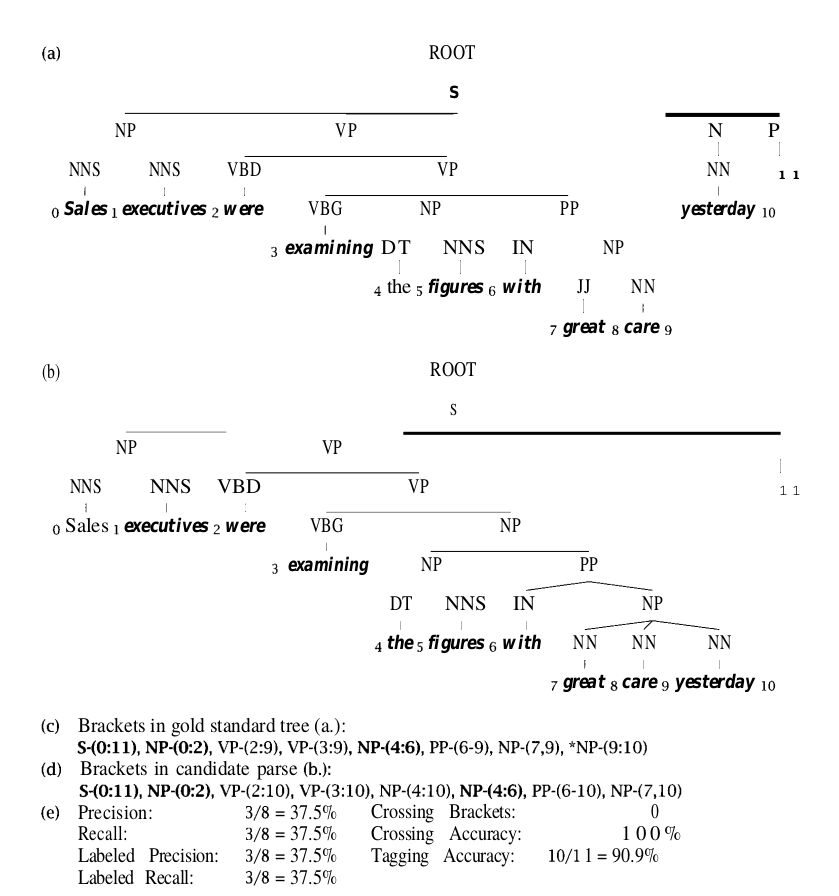
\includegraphics[width=\textwidth]{imagens/fig_demo_parseval.png}
    % \includesvg[width=.8\textwidth]{demo}
    % \includesvg{imagens/cintil_pcfg}
    \caption[Demonstração do funcionamento do PARSERVAL]{Demonstração do funcionamento do PARSERVAL. Extraido de \citeonline[p~433]{Manning1999FoundationsNLP}. Note que o nó NP-(9:10) (\textit{yesterday}), ao ser posicionado como filho do nó NP-(7:10), torna todos os nós acima dele também errados.}
    \label{fig:demo_parseval}
\end{figure}
\end{center}

Nesse contexto, o cálculo do F-MEASURE se dá utilizando a mesma Equação \ref{eq:f_score}.

Algumas críticas podem ser feitas à esse sistema. \citeonline{constParsEvalYT} demonstra que essa medida é muito sensível à propagação de erros em cascata. Ou seja, um constituinte mal colocado num nível mais baixo da árvore faz com que todos os nós acima dela também estejam errados, reduzindo muito a pontuação. \citeonline{parserEvalSecret} também nota que \textquote{\textit{The problem of standard Parseval is that it counts nodes as the same regardless of the underlying structure they dominate}}
\footnote{\textquote{O problema do PARSERVAL padrão é que ele conta nós como os mesmos, independente da estrutura subalterna que estes dominam}. Tradução própria.}.

Isto pode ser melhor observado na Figura \ref{fig:demo_parseval}. Numa sentença $W=[w_0 \ldots w_n]$, para $w_j$ palavras, os nós dá árvore são identificados por $P-(i:f)$, sendo $P$ a \textit{POS tag}, $i$ o inicio da \textit{abrangência} do nó, e $f$ o final. Nós com mesma \textit{POS} são identificados pela ordem de aparecimento na árvore, e pela abrangência. Por \textit{abrangência}, refere-se ao alcance de todos os seus descendentes. Assim, na árvore \ref{fig:demo_parseval}[a], o primeiro VP é representado por $VP-(2:9)$ por englobar a sentença de \textquote{\textit{were}} a \textquote{\textit{care}}. Note que, ao posicionar o último NP, referente à \textquote{\textit{yesterday}}, a árvore candidata o marca como $NP-(7:10)$, em contraste com o \textquote{padrão-ouro}, que deveria ser $NP-(9:10)$. Isto faz com que, não só este nó esteja errado, como todos os nós acima dele, fazendo com que os valores de LP, LR e, por fim, F1 sejam afetados negativamente.